\documentclass[12pt]{article}


\usepackage{graphicx}
\usepackage{fullpage}

\setlength{\parindent}{0pt}
\setlength{\parskip}{1ex plus 0.5ex minus 0.2ex}

\title{CSE 834 Low Pass Filter}
\author{Derek Weitzel \& Yutaka Tsutano}

\begin{document}
\maketitle

\section{Introduction} \label{sec:introduction}


\section{Introduction}
Low pass filters are used in many applications from noise filtering to RF modulation.  Low pass filters are well understood, and include logically simple components: registers, adders, and multipliers.  In this project, we will design a low power low pass filter using the VHDL and the Cadence hardware designer.  We will include optimizations for power such as reducing components and reducing transitions.

In section \ref{sec:design}, we will discuss our design philosophy and design decisions.  In section \ref{sec:implementation} we will describe how we constructed the components and connected them.  Finally, in section \ref{sec:conclusion}, we will discuss problems we experienced in our design and the tools we used.


In this project, we will create a 16 bit low pass filter.  This filter is similar to those used in audio processing.  The specific properties of the filter where picked to simplify the design.

For each clock period, the circuit will:
\begin{itemize}
\item Shift the registers.  This will pop the last register's value, and save the data\_in value to the first register.
\item Calculate the convolution of the values inside the 8 registers.
\end{itemize}

The coefficients are fixed, therefore they will be constant in the multipliers, simplifying the design.  The input will be 1 bit for the clock, and 16 bits of input data.  The output will be the 16 bit output.  The format of the input and output will be Q15.  The multipliers  and registers will be done in VHDL in order to simplify design.

\begin{table}[ht]
\centering
\begin{tabular}{l | l | c}
\hline
Input/Output & Description & Bits \\
\hline \hline
Input & Clock & 1 \\
Input & Data In & 16 \\
Output & Convolution & 16 \\
\end{tabular}
\end{table}

We will tackle power concerns by optimizing the tree of adders (see Figure \ref{fig:diagram}).  Since we have a constant number of adders, we can create a large adder that will be able to minimize redundant gates.  Further, because of the symmetric property of the filter, we can minimize the number of multipliers by adding symmetric registers, then multiplying by the coefficient.  

\section{Timeline}

11/2 - 11/8: Registers and Multipliers \\
11/8 - 11/23: Optimized Adder \\
11/23 - 12/2: Report - Finalizations \\

\section{Filter Properties}
These are the specific filter properties that where used to calculate the Coefficients seen in Table \ref{tab:coefficients}.

Sampling Frequency Fs = 8194 Hz \\
Cut-off Frequency = 2048 Hz \\
FIR (Lowpass Filter with Hamming Window) \\

\begin{table}[ht]
\centering
\begin{tabular}{ c | r }
\hline
Coeffiecient & Value \\
\hline \hline
$C_0$ & -1.55107884796477e-18 \\
$C_1$ & -0.022663985459552 \\
$C_2$ & 1.04697822237622e-17 \\
$C_3$ & 0.273977082565524 \\
$C_4$ & 0.497373805788057 \\
$C_5$ & 0.273977082565524 \\
$C_6$ & 1.04697822237622e-17 \\
$C_7$ & -0.0226639854595526 \\
$C_8$ & -1.55107884796477e-18 \\
\end{tabular}
\caption{Coefficient values}
\label{tab:coefficients}
\end{table}


\section{Design}
\label{sec:design}

\subsection{Q15 Format} \label{sec:q15}

For our filter design, fixed format number format called Q is used. Unlike floating point numbers, Q-format numbers require only standard integer ALU to perform rational number calculations. This means that we do not need to add an FPU to our design which requires additional power.

Q format numbers are represented using the Q notation which is written as Q$m,n$ where $m$ is the number of bits set aside to designate the two's complement integer portion of the number, and $n$ is the number of bits used to designate the fractional portion of the number.

In our case, we use simplified notation Q$n$ since we assume that the numbers are normalized into the range of $[-1, 1)$. Notice that this assumption does not affect the generality of the filter, but it simplifies the multiplication operation because the multiplication result never exceeds the range of $[-1, 1)$.

\begin{figure}[ht]
	\centering
	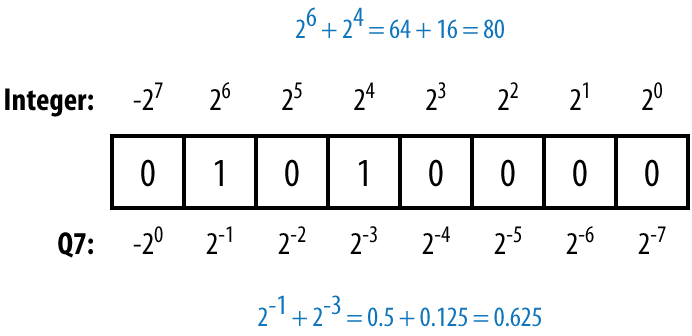
\includegraphics[scale=1.5]{images/q7}
	\caption{Comparison between integer and Q7 format.}
	\label{fig:q7}
\end{figure}

Figure \ref{fig:q7} shows the comparison between two's complement integer and Q7 numbers. The only difference between the two is the weight assigned for each bit.

\subsection{Filter Characteristics}

\begin{table}[ht]
\centering
\begin{tabular}{ c | r | r }
\hline
Coeffiecient & Value & Q15 \\
\hline \hline
$C_0$ & -0.022663985459552   & \texttt{1111110100011010} \\
$C_1$ & 1.04697822237622e-17 & \texttt{0000000000000000} \\
$C_2$ & 0.273977082565524    & \texttt{0010001100010001}\\
$C_3$ & 0.497373805788057    & \texttt{0011111110101001}\\
$C_4$ & 0.273977082565524    & \texttt{0010001100010001}\\
$C_5$ & 1.04697822237622e-17 & \texttt{0000000000000000} \\
$C_6$ & -0.022663985459552   & \texttt{1111110100011010} \\
\end{tabular}
\caption{Coefficient values}
\label{tab:coefficients}
\end{table}

The coefficients for the filter is shown in Table \ref{tab:coefficients}. These values were computed using Filter Design \& Analysis Tool (Figure \ref{fig:matlab}) in Matlab Signal Processing Toolbox which is one of the most widely used filter design tool in the industry. We have chosen FIR filter with Hamming window with order of 8. This filter is also one of the most widely used in the industry and has straight-forward characteristic.

\begin{figure}[ht]
	\centering
	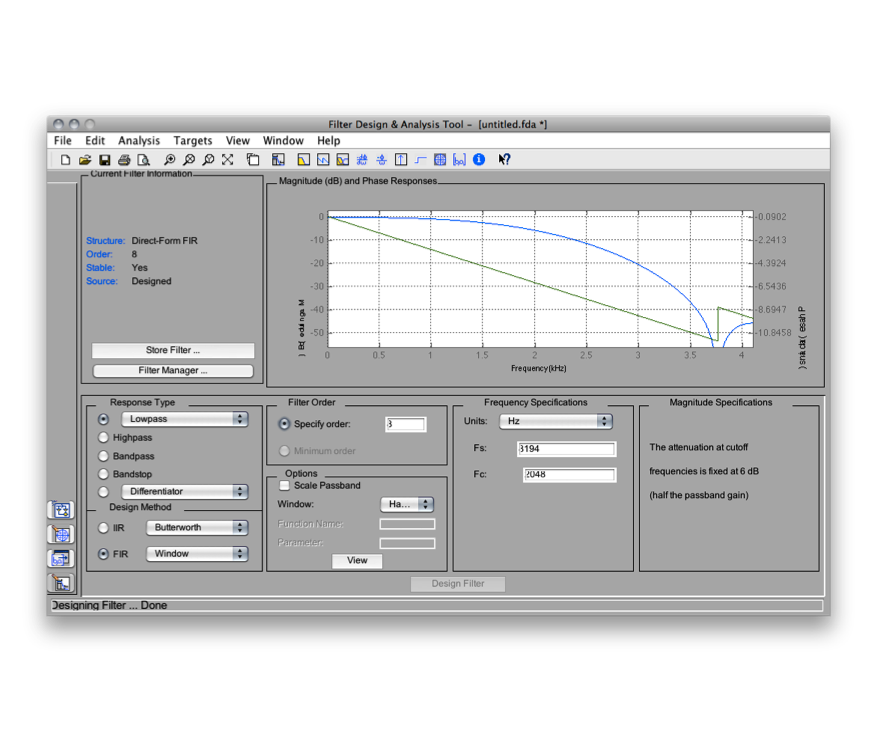
\includegraphics[scale=1]{images/matlab}
	\caption{Matlab Filter Design \& Analysis Tool.}
	\label{fig:matlab}
\end{figure}

\subsection{Input \& Output}
The input and output of our design are shown in Table \ref{table:inputoutput}.  The external clock will allow us to connect to arbitrary clocked external input, as long as it meets the timing requirements of our design.  The 16 bit input and output are in the Q15 format described in Section \ref{sec:q15}.  The Q15 format is an industry standard, hence we expect that these required input formats are reasonable.

\begin{table}[ht]
\centering
\begin{tabular}{l | l | c}
\hline
Input/Output & Description & Bits \\
\hline \hline
Input & Clock & 1 \\
Input & Data In & 16 \\
Output & Convolution & 16 \\
\end{tabular}
\caption{Description of input and output to the filter.}
\label{table:inputoutput}
\end{table}



\subsection{Power Optimization}

% Duplicate multipliers
We will optimize power by removing duplicate multipliers.  These duplicate multipliers are created because the filter is symmetric, therefore an adder can be used remove an adder.  In the naive filter, shown in Figure \ref{fig:naivefilter}, the constant is multiplied against each register value.  Since the constants are symmetric, ie $C0$ is the same as $C6$, this can be optimized using the associative rule.  In Figure \ref{fig:optimizedfilter}, you can see that we have removed 3 of the multipliers.  Instead, we add the values in the registers before multiplying the constants.  This eliminates 3 large and power draining multipliers.  It also simplifies the final adder from 7 input to 4.


\begin{figure}[ht]
\centering
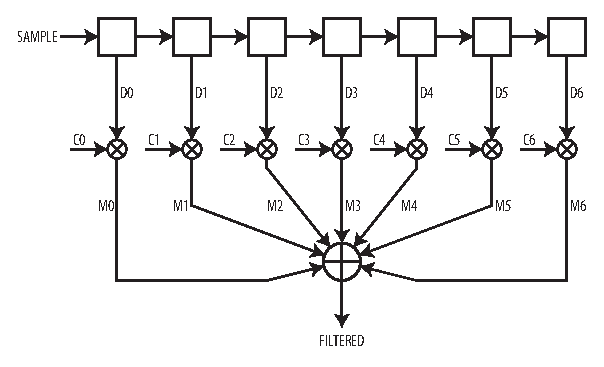
\includegraphics[width=5in]{images/filter_normal}
\caption{Naive filter implementation.}
\label{fig:naivefilter}
\end{figure}

\begin{figure}[ht]
\centering
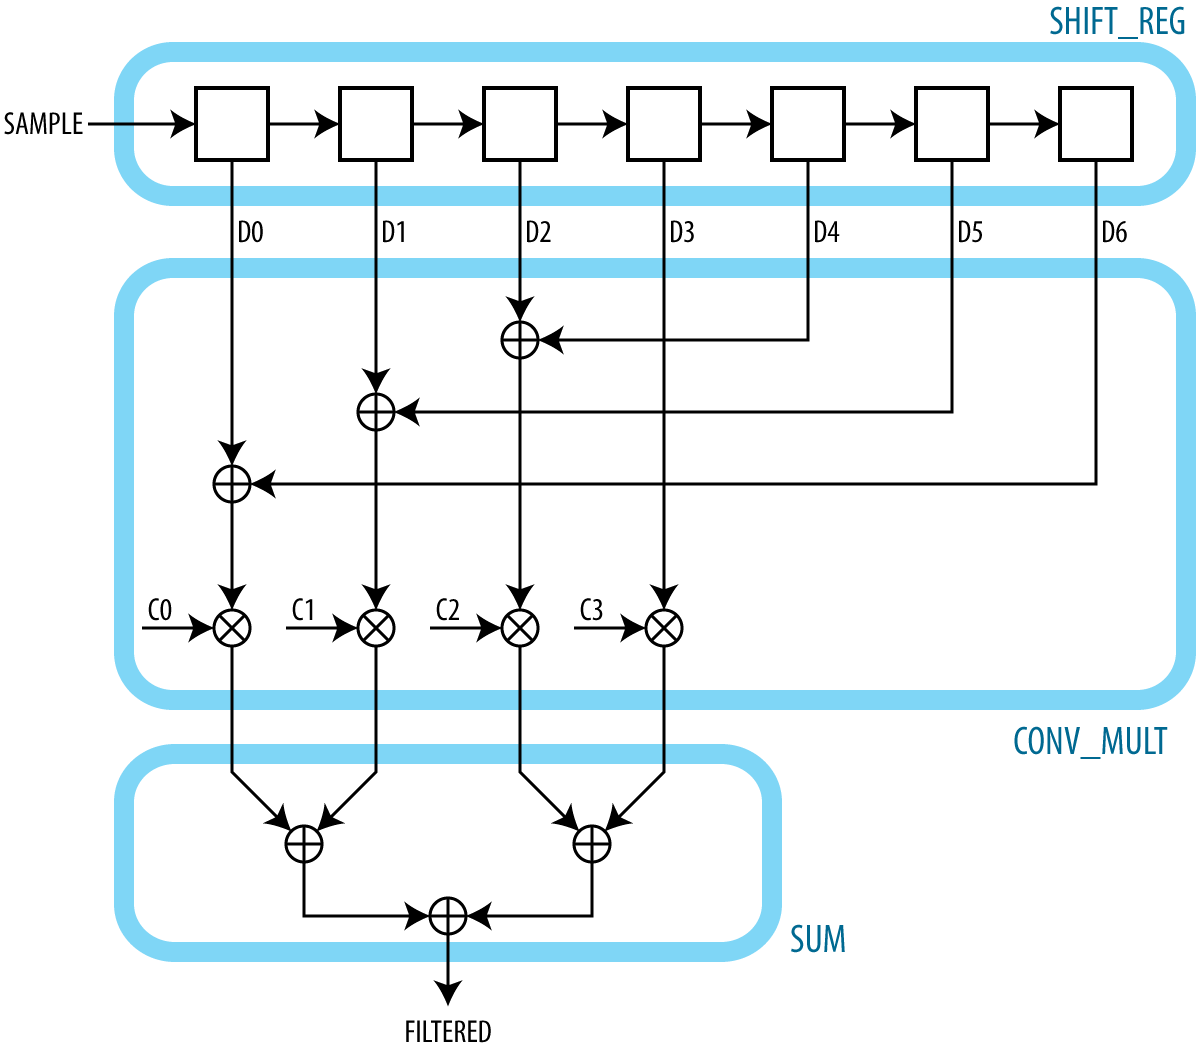
\includegraphics[width=5in]{images/filter_filtered}
\caption{Optimized filter implementation.}
\label{fig:optimizedfilter}
\end{figure}

% Ripple carry adders
The adders shown at the bottom of Figure \ref{fig:optimizedfilter} are frequently changing as the final value is stabilized through the convolution hardware above.  Therefore, it is important that this hardware is optimized for power.  With reducing the number of transistors as our goal, we designed ripple-carry adders to do the final addition.  The ripple-carry adders have less hardware than the optimized version that VHDL synthesized when doing a `+'.  Also, the ripple carry adders will localize any transition to only the nodes that require it.

Compare the ripple carry to propagate/carry (PG) adders that are designed to optimize latency.  The PG adders have significantly more hardware since it has to pre-calculate propagates and carries.  

We also attempted to use a clock-gated D flip flop seen in Figure \ref{fig:gateclocked}.  While doing simulations of the VHDL, we discovered that this design was flawed.  When the clock was high, Q stabilized to the value of D.  This is because the XOR gate with the clock and the D input would cause the `clock' input to the flip flop to change, therefore causing it to save the input.  The clock-gated D flip-flop acted as a latch.  We did not use this optimization in the final design.


\begin{figure}[ht]
\centering
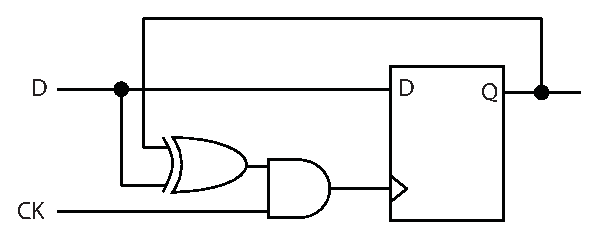
\includegraphics[width=5in]{images/clockgating}
\caption{Clock gating low power flip-flop (Credit: Sharad Seth).}
\label{fig:gateclocked}
\end{figure}





\section{Implementation} \label{sec:implementation}
\subsection{VHDL Design}
We decided to design our filter using as much HDL as possible.  Therefore, every component is written in VHDL, and are synthesized for the final design. The VHDL is separated into components listed below.  These components are then sythensized using the rc cadenced synthesizer. 

Separate components:
\begin{itemize}
\item D\_FF
\item CONV\_MULT
\item ADD16
\item FullAdder
\end{itemize}

\subsection{Functional Verification}
To verify the correctness of the VHDL design files, we have written a C++ program that generates test cases. This program first generates test input with random noise. Then it computes the output using the equivalent filter algorithm in Q15 format. The result is stored in a text file (Appendix \ref{lst:testcase.txt}) which can be read by a VHDL testbench \texttt{filter\_tb.vhd} (Appendix \ref{lst:filter_tb.vhd}).

\begin{figure}[ht]
	\centering
	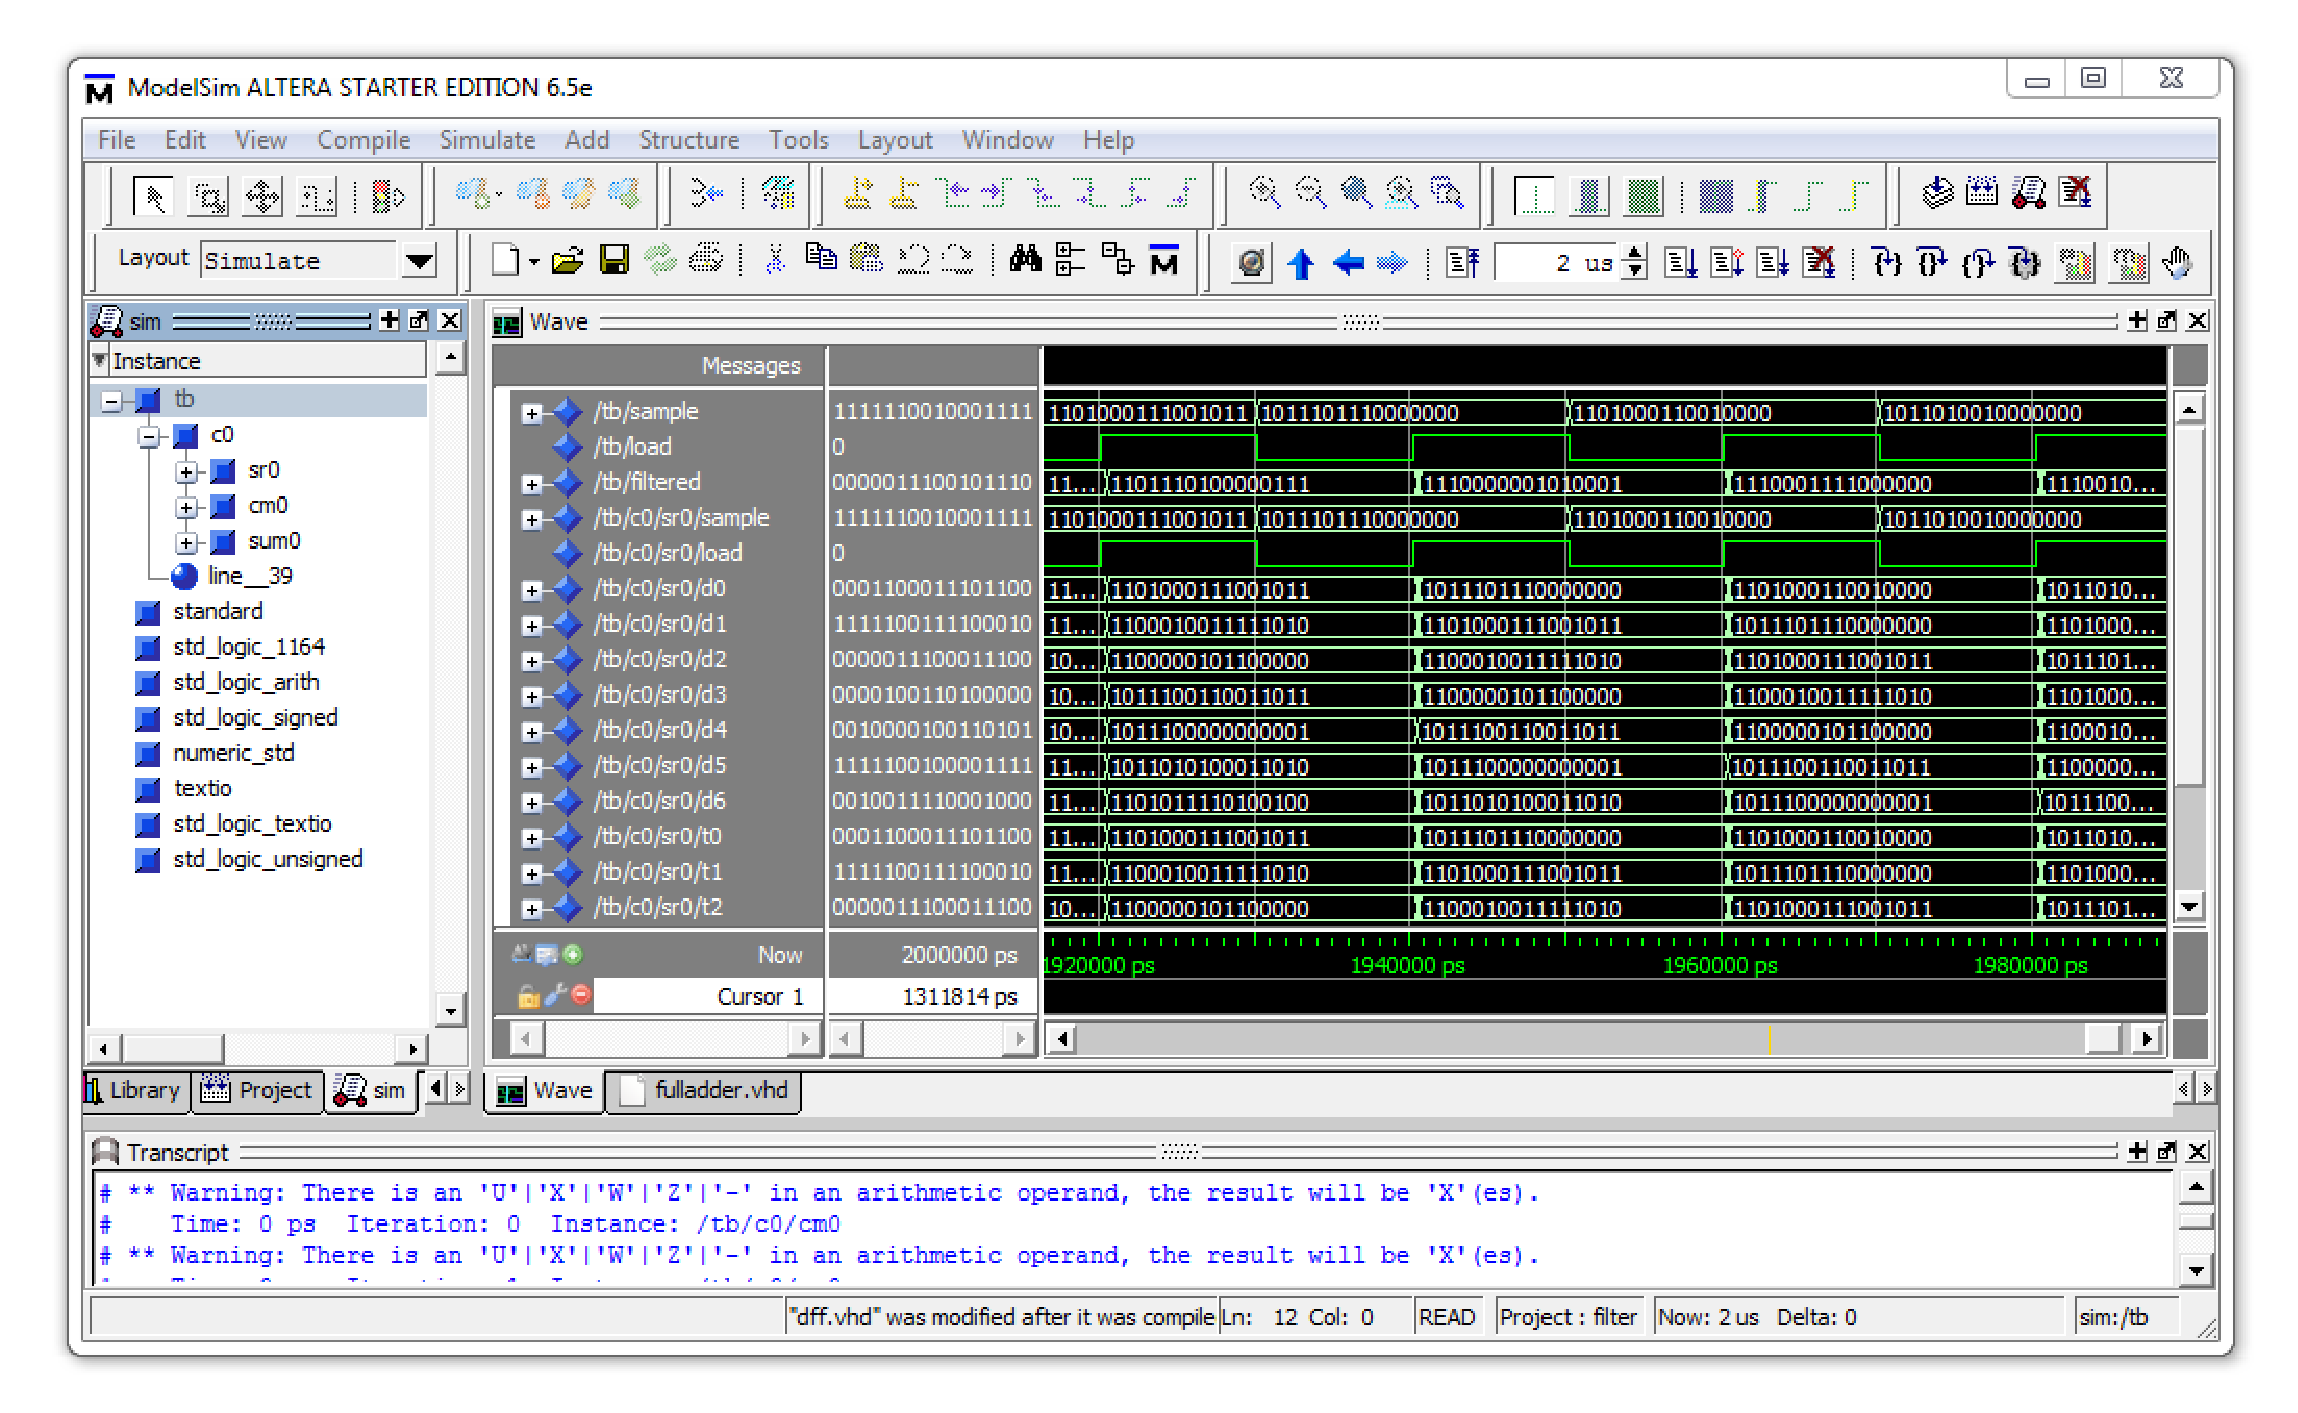
\includegraphics[width=6.5in]{images/modelsim}
	\caption{ModelSim from Mentor Graphics was used for VHDL simulation.}
	\label{fig:q7}
\end{figure}

For VHDL simulation, we used ModelSim from Mentor Graphics. This tools loads and compiles all VHDL files including the test bench, then shows the waveform and output to the window. Our testbench file follows the VHDL standard and prints the results into a text file, so it should work on other environments other than ModelSim.

We verified that the every bit of the C++ program output and VHDL testbench output matched, therefore the VHDL should be correct with high probability.


\subsection{Synthesis}



\subsection{Final Layout \& Routing}


\section{Conclusion} \label{sec:conclusion}

% Conclusion

In this project, we created a power optimized low pass filter.  We avoid using a floating point unit by utilizing the Q15 format.  The filter is symmetric, allowing for optimizations.  The input and output is kept simple.    The power optimizations where done at design time using the algorithmic level.  The components where developed in VHDL.  The design was verified both at the functional level with a C++ program, and using the VHDL through a simulator.  The components where synthesized using the Cadence tools.  Finally, the layout was done using the autorouter in Cadence.



\if 0

\section{Overview}
In this project, we will create a 16 bit low pass filter.  This filter is similar to those used in audio processing.  This specific properties of the filter where picked to simplify the design.

For each clock period, the circuit will:
\begin{itemize}
\item Shift the registers.  This will pop the last register's value, and save the data\_in value to the first register.
\item Calculate the convolution of the values inside the 8 registers.
\end{itemize}

The coefficients are fixed, therefore they will be constant in the multipliers, simplifying the design.  The input will be 1 bit for the clock, and 16 bits of input data.  The output will be the 16 bit output.  The format of the input and output will be Q15.  The multipliers  and registers will be done in VHDL in order to simplify design.

\begin{table}[ht]
\centering
\begin{tabular}{l | l | c}
\hline
Input/Output & Description & Bits \\
\hline \hline
Input & Clock & 1 \\
Input & Data In & 16 \\
Output & Convolution & 16 \\
\end{tabular}
\end{table}

We will tackle power concerns by optimizing the tree of adders (see Figure \ref{fig:diagram}).  Since we have a constant number of adders, we can create a large adder that will be able to minimize redundant gates.  Further, because of the symmetric property of the filter, we can minimize the number of multipliers by adding symmetric registers, then multiplying by the coefficient.  

\section{Timeline}

11/2 - 11/8: Registers and Multipliers \\
11/8 - 11/23: Optimized Adder \\
11/23 - 12/2: Report - Finalizations \\

\section{Filter Properties}
These are the specific filter properties that where used to calculate the Coefficients seen in Table \ref{tab:coefficients}.

Sampling Frequency Fs = 8194 Hz \\
Cut-off Frequency = 2048 Hz \\
FIR (Lowpass Filter with Hamming Window) \\

\begin{table}[ht]
\centering
\begin{tabular}{ c | r }
\hline
Coeffiecient & Value \\
\hline \hline
$C_0$ & -1.55107884796477e-18 \\
$C_1$ & -0.022663985459552 \\
$C_2$ & 1.04697822237622e-17 \\
$C_3$ & 0.273977082565524 \\
$C_4$ & 0.497373805788057 \\
$C_5$ & 0.273977082565524 \\
$C_6$ & 1.04697822237622e-17 \\
$C_7$ & -0.0226639854595526 \\
$C_8$ & -1.55107884796477e-18 \\
\end{tabular}
\caption{Coefficient values}
\label{tab:coefficients}
\end{table}


%\begin{figure}[ht]
%\centering
%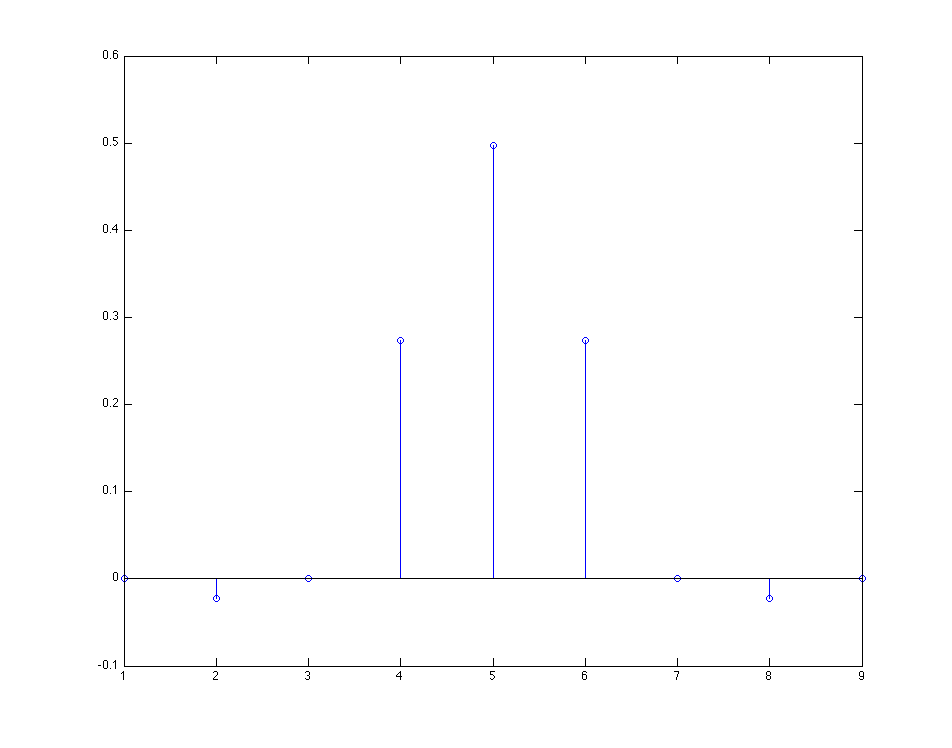
\includegraphics[scale=0.55]{../coeffs.png}
%\caption{Plot of coefficients.  Notice the symmetry.}
%\label{fig:plotcoefficients}
%\end{figure}

%\begin{figure}[ht]
%\centering
%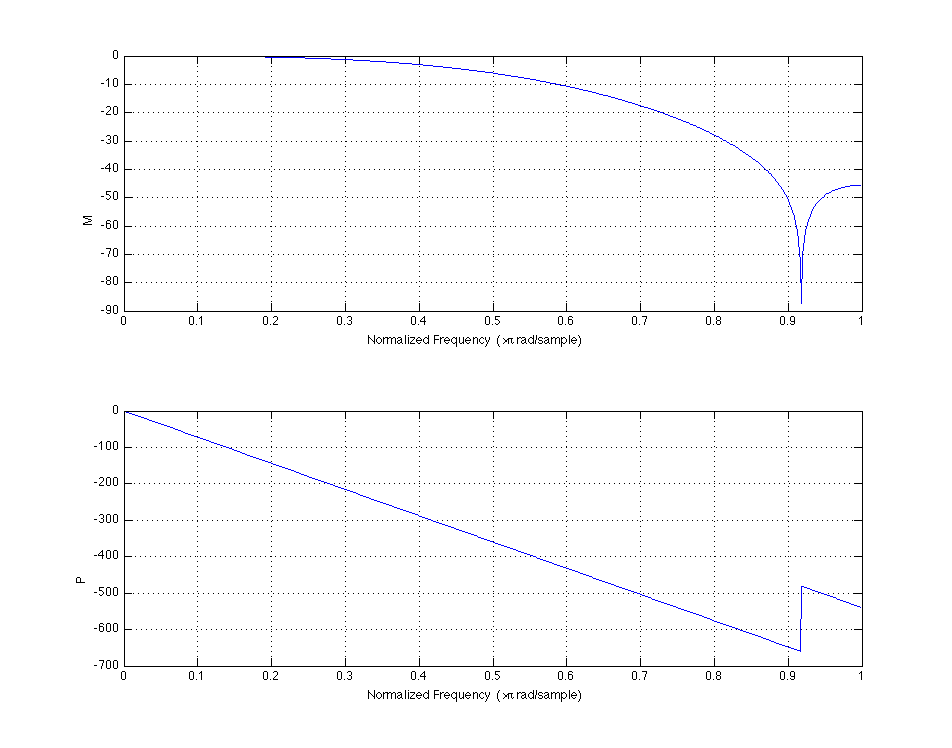
\includegraphics[scale=0.55]{../filter_design.png}
%\caption{Plot of filter characteristics}
%\label{fig:characteristics}
%\end{figure}

%\begin{figure}[ht]
%\centering
%\includegraphics[scale=0.55]{../Diagram.png}
%\caption{Logical diagram of the data flow.}
%\label{fig:diagram}
%\end{figure}

\fi

\end{document}
